\chapter{Introduction}

In lean/agile product development, it is necessary to have formalized user feedback loops in place, to measure product performance against various (quantitative) metrics. Such feedback loops obtain the information and statistics regarding user engagement and interaction with the developed product. Are the users using it the way the creator imagined or did they find any other means of utilizing it? What stops the users from doing the task they intended to do? Do they get everything they need, and at the same time, does the creator get what was expected? In other words, are the dominant means of usage incentive compatible for the users? 

Not only do the current solutions for gathering such user data for both quantitative and qualitative metrics work out-of-the-box with low-level semantics only (everything is a general activity using a general resource), but they also tend to run on somebody else's servers. What if the product developer is in a highly regulated market, such as pharmaceuticals, and has to own all user data? How can the current solutions' space be utilized and tweaked in order to fit such a schema?

\subsection*{Data Disconnectivity}

The most problematic issue in large corporations is the semantic disconnectivity of the data. This occurs when data is collected ad hoc without any set direction or goal to be achieved. It may physically be all there, however nobody knows what it's worth or how it should be connected in order for it to make sense and drive value. Do I have good data or do I just have petabytes of useless log trace? Am I gathering information on what the application was intended to do or am I only filling the database with irrelevant garbage information. Most importantly though, am I gathering the information I need in a consistent fashion that corresponds to the domain of the shareholders?

Let's draw an analogy here and let me illustrate the problem with a real-world example.

\newpage

\subsection*{Example}

\begin{figure}[!ht]
	\centering
	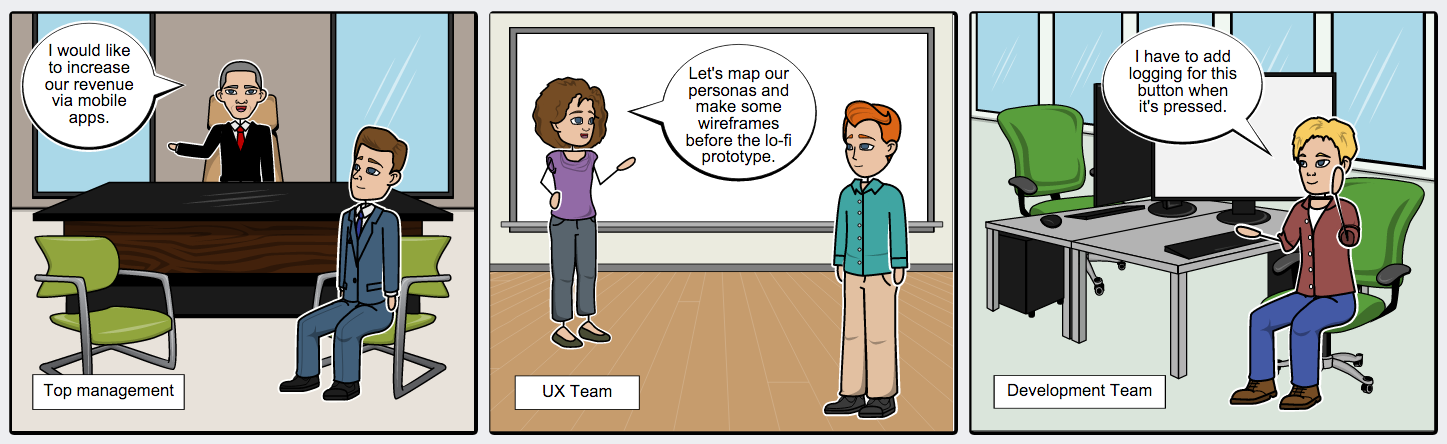
\includegraphics[width=0.9\textwidth]{figures/01_introduction/storyboard}
    \caption{Real-World Example}
\end{figure}

This situation is mainly caused by:

\begin{enumerate}
	\item Top management comes with a need to increase revenue via mobile devices.
	\item Project management team takes over and breaks it down to user-stories, tasks etc.
	\item Project management team asks the UX team, the mobile applications team and the backend team to perform their tasks in order to bring the product to life.
	\item By the time product development is spread across three different teams, it is very much likely that each team will create their own jargon for every activity performed in the product.
		\begin{itemize}
			\item The UX team is driven by the larger picture so they tend to refer to objects in a highly abstract way.
			\item The backend team is driven by the inner processes happening between the \\ database and the REST API, so they speak their precise technical language.
			\item The mobile applications team is somewhere in-between, but never really aligned with either of the other teams.
		\end{itemize}
	\item When the product is delivered, the project management team has a really hard time comparing the reported results with the top management's primary goals. Plus, the larger the teams are, the worse the situation actually gets.
\end{enumerate}

This isn't a problem of poor project management. The company can use the best project management tools on the market and have the smartest people working on their teams and still encounter this problem on a daily basis. This is a larger problem resulting from the lack of intersection between different domains (Management, UX, Development, DevOps).

\newpage

\section{Work Environment}

The context of this work is a large company, operating in a regulated market, where products are developed across multiple departments varying not only in size and experience, but also in project management approach - traditional and agile methods. Both methods implemented in the organization have a common denominator: measured KPIs to indicate the status of the work.

\subsection{Key Performance Indicators}

Each department/team/person has very specific Key Performance Indicators (= KPIs) \cite{weber2005key} that represent the value of their work. Even products have their KPIs - "How much value has this product brought?", "How much time is this product saving us?", etc.

\subsection{Software Development Life Cycle}

Software Development Life Cycle (= SDLC) is a standardized traditional and formalized approach to developing a software product for regulated markets. It enables companies to follow specific steps in order to get their software product certified for use in constrained environments. It is used not for the sake of bureaucracy, but to protect the customers and increase the level of traceability of a problem, should one ever occur.

\subsection{Agile Development Methodologies}

In the modern era of software development, it has become "cool" to not follow traditional waterfall models and to adopt agile methodologies, such as scrum or kanban. For many years these were found exclusively in start-ups. But because time and time again, research \cite{947100} has shown that agile methodologies do impact the level of productivity and innovation, larger companies are working on adopting them in their constrained context as well. This thesis operates in such a place, where agile methodologies are being deployed across the whole innovation department.

\section{Personal Interviews}

In order to find out what needs there are, I have conducted several interviews with leaders of various departments. These are their reactions to what bothers them about product monitoring during the development phase:

\begin{enumerate}
		\item Associate Director, Applied Technology
		\begin{itemize}
				\item[] "The real problem I see is the fact that all the information I need is on somebody else's server. We can't store any sensitive, let alone confidential information \emph{somewhere} with some random vendor. It's actually illegal in some countries. Unfortunately, sometimes sensitive data is exactly what we need to obtain from the applications to make an informed decision."
		\end{itemize}	

		\item Associate Director, Mobile and Web
		\begin{itemize}
				\item[] "Our needs for tracking KPIs are variable throughout time and unfortunately the current tools we use are quite inflexible. Because we are in a regulated market, each change that requires a new build of an application takes a longer period of time. And time \emph{is} money."
		\end{itemize}				
		
		\item Mobile Application Development Lead
		\begin{itemize}
				\item[] "I have noticed that one of the biggest obstacles is how should we name what we measure. I have no vocabulary to help me during the development. The only thing we have is a robust Google Analytics toolkit that only allows us to gather low-level actions. We can log that a button was pressed, but what do we name such action? "Button pressed"?"
		\end{itemize}
		
		\item UX Lead
		\begin{itemize}
				\item[] "Our team looks at the high-level needs. We are trying to make the user activities in an application as smooth as possible. When we design a low-fidelity prototype, we know what we want to measure. Having the opportunity to add a high-level KPI would help us a lot in order to gather feedback for our prototypes. We are not programmers, we don't know how to add it to the code, but I would love the idea of including what to measure along with the prototype."
		\end{itemize}
\end{enumerate}

\section{Scope of Work}

First, I will present the context of agile software development in a regulated market. Then I will take a look at the current tracking solutions being used in mobile development (the focus is on iOS development, but most of the tools are multiplatform solutions). I will examine and analyze their strengths and weaknesses. 

Next I will propose a workflow to fit the needs of a larger company with multiple departments, operating in a regulated market. I will utilize existing tools and build on top of them in order to drive value without reinventing the wheel.

Lastly, I will develop a working PoC (Proof of Concept), verify its functions through user testing and further discuss with the stakeholders whether or not it is the correct path to take in order to unite all departments and connect the dots in the data.